\section{Menù principale}
\subsection{Main Activity}
Una volta effettuata la registrazione o login l'applicazione mostra la schermata principale contenente i veicoli dell'utente già inseriti oppure una scritta centrale "Carica un veicolo" nel caso non ve ne siano.
 \begin{figure}[H] 
	\centering 
	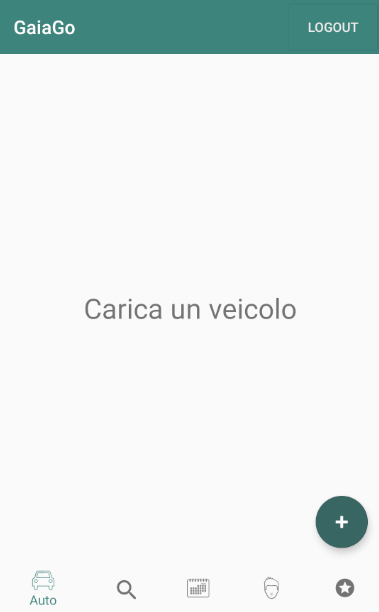
\includegraphics[width=0.5\textwidth]{res/images/main_activity_vuota.png}\\
	\caption{Main Activity}
	\label{Login}
\end{figure}
\pagebreak
\subsection{Logout e Barra di Navigazione}
Andiamo ora ad analizzare due parti fondamentali presenti in tutte e cinque le activity\glosp principali:
\begin{itemize}
	\item \textbf{Logout}: presente in alto a destra, permette all'utente di scollegare l'account in uso da \textit{Gaiago} e riporta alla schermata di login;
	\\\\
	  \begin{figure}[H] 
	 	\centering 
	 	
\includegraphics[width=0.5\textwidth]{res/images/logout.png}\\
	 	\caption{Bottone di Logout}
	 	\label{Login button}
	 \end{figure}
 Una volta premuto compare il seguente dialog\glosp per chiedere la conferma.
 \\\\
 \begin{figure}[H] 
 	\centering 
 	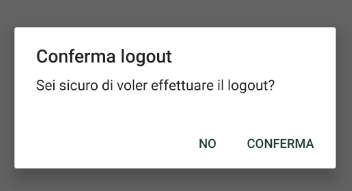
\includegraphics[width=0.5\textwidth]{res/images/logout_press.png}\\
 	\caption{Dialog Logout}
 	\label{Logout_press}
 \end{figure}
 	\item  \textbf{Barra di Navigazione}: presente in basso, permette all'utente di muoversi tra le varie funzionalità principali di \textit{GaiaGo}.
 	\\\\
 	  \begin{figure}[H] 
 	  	\centering 
 	  	
\includegraphics[width=0.5\textwidth]{res/images/barra_navigazione.png}\\
 	  	\caption{Barra di Navigazione}
 	  	\label{Barra di navigazione}
 	  \end{figure}
\end{itemize}
\pagebreak

\subsection{Gestione veicoli}
La gestione dei veicoli si trova nell'attività principale, nella barra di navigazione è rappresentata da un automobile stilizzata e con la scritta "Auto" se ci si trova al suo interno.
 \begin{figure}[H] 
	\centering 
	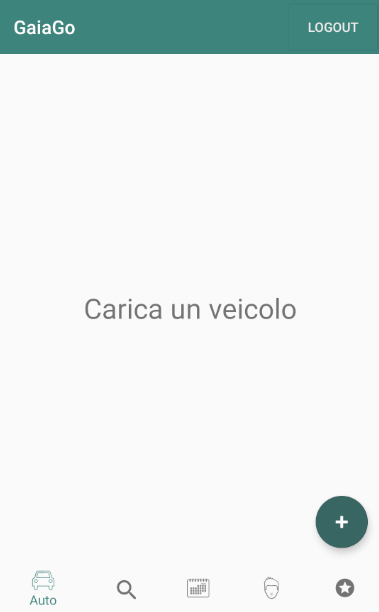
\includegraphics[width=0.5\textwidth]{res/images/main_activity_vuota.png}\\
	\caption{Main Activity}
	\label{main}
\end{figure}
\pagebreak
\subsubsection{Inserimento veicolo}
All'utente è consentito di caricare i propri veicoli all'interno di \textit{GaiaGo}, per fare ciò, dalla schermata dove sono presenti i propri veicoli(o non ve ne sono perché ancora da caricare), si preme il bottone verde contrassegnato da una "+" bianca.
Si viene portati ad una attività secondaria la quale permette l'inserimento dei dati del veicolo seguenti:
\begin{itemize}
	\item \textbf{Foto}: è necessario inserire una foto del proprio veicolo per renderlo riconoscibile agli altri utenti, per fare ciò si preme il bottone verde contrassegnato da una "+" bianca.
	 \begin{figure}[H] 
		\centering 
		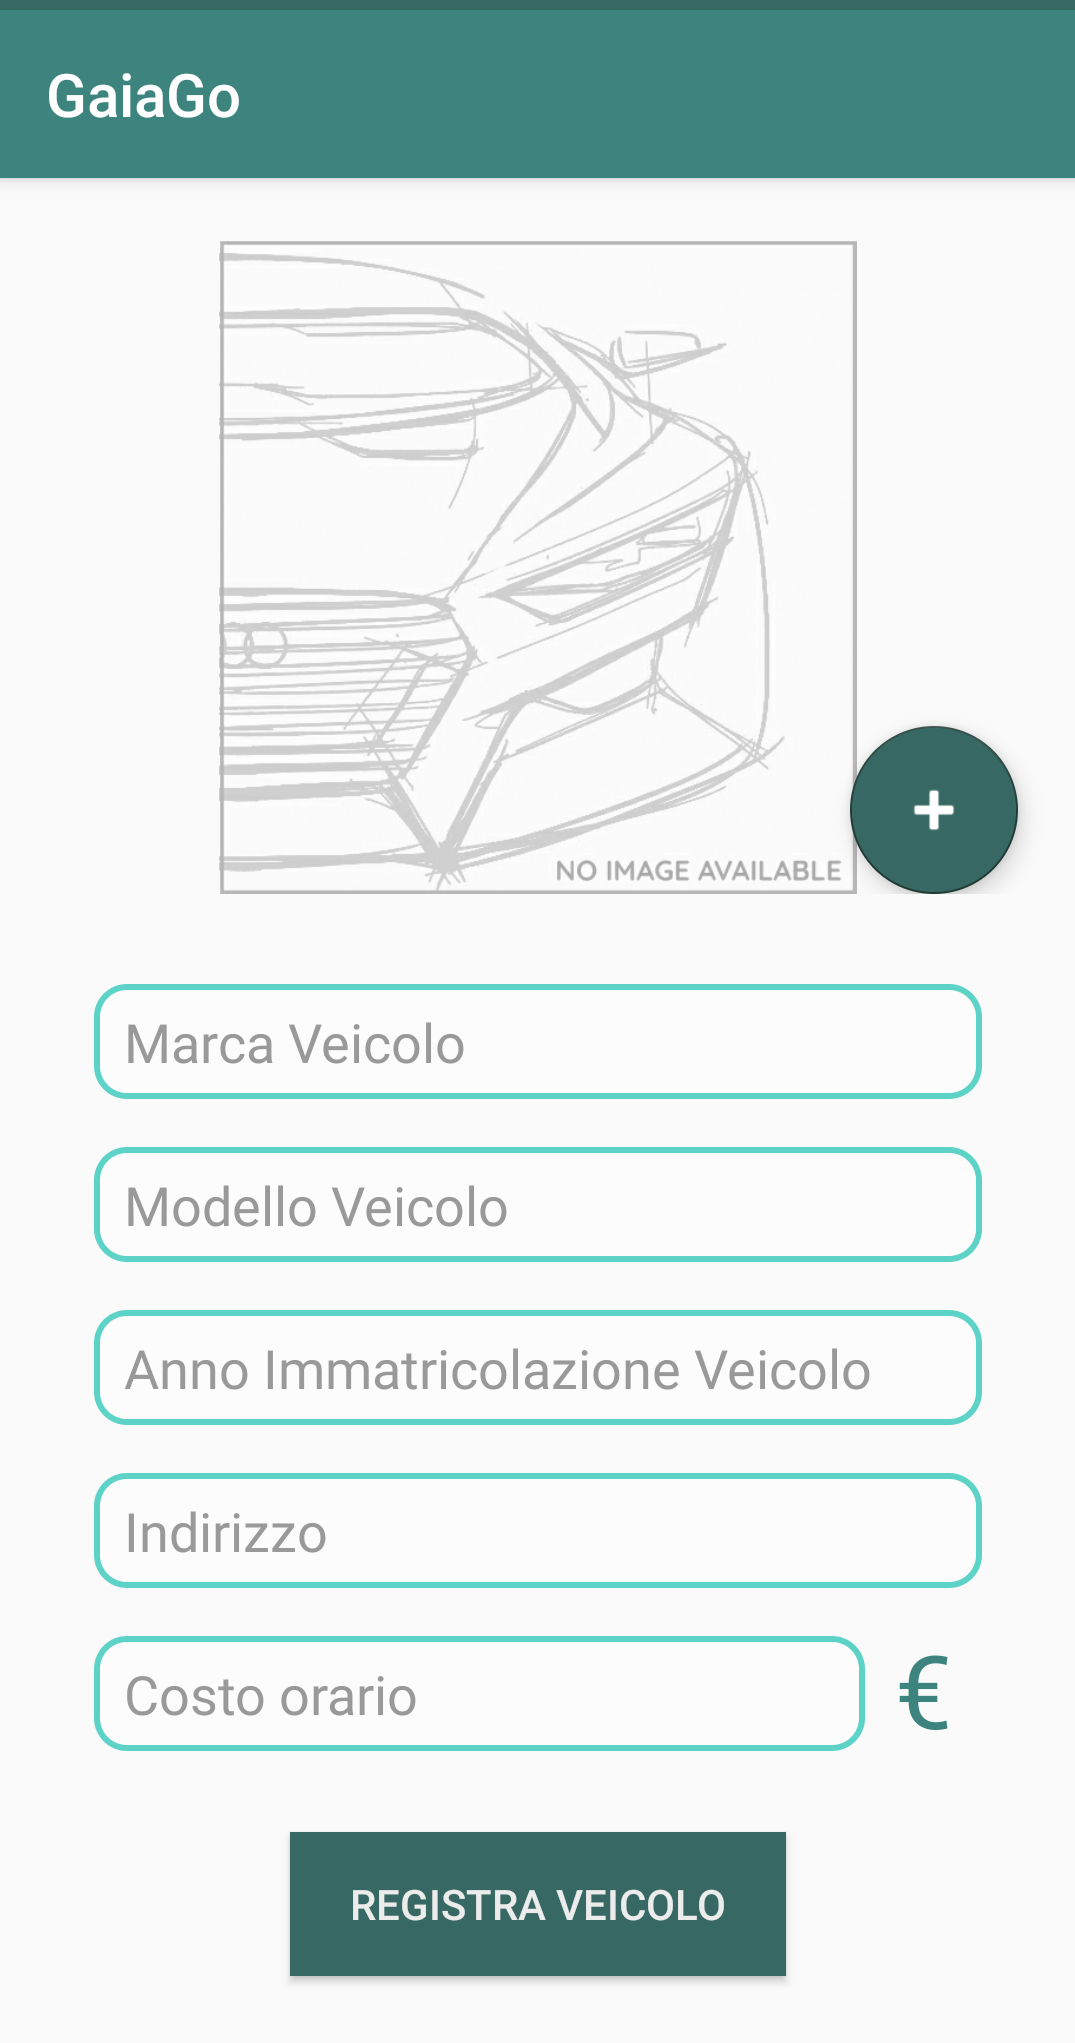
\includegraphics[width=0.5\textwidth]{res/images/caricamento_veicolo.png}\\
		\caption{Inserimento veicolo}
		\label{ins}
	\end{figure}
\pagebreak

Una volta premuto il pulsante si deve scegliere da dove caricare l'immagine e successivamente si preme sull'immagine da caricare;
 \begin{figure}[H] 
	\centering 
	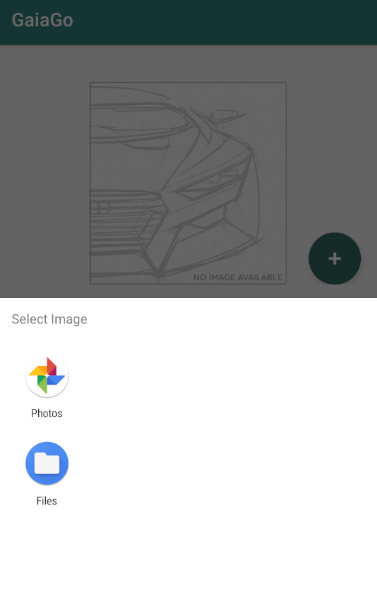
\includegraphics[width=0.5\textwidth]{res/images/caricamento_veicolo_bottone_premuto.png}\\
	\caption{Scelta immagine}
	\label{img}
\end{figure}
\pagebreak

\item \textbf{Marca}: in questa sezione si sceglie la marca del proprio veicolo, per velocizzare ciò è reso disponibile un algoritmo di ricerca dinamico per l'auto completamento;
 \begin{figure}[H] 
	\centering 
	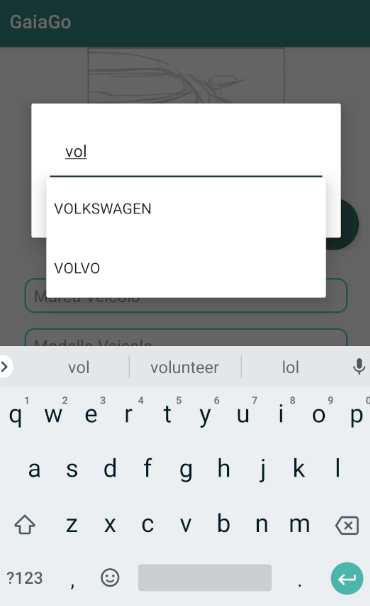
\includegraphics[width=0.5\textwidth]{res/images/marca_auto.png}\\
	\caption{Scelta marca}
	\label{marca}
\end{figure}
\pagebreak

\item \textbf{Modello}: in questa sezione si sceglie il modello del proprio veicolo, per velocizzare ciò è reso disponibile un algoritmo di ricerca dinamico per l'auto completamento;
 \begin{figure}[H] 
	\centering 
	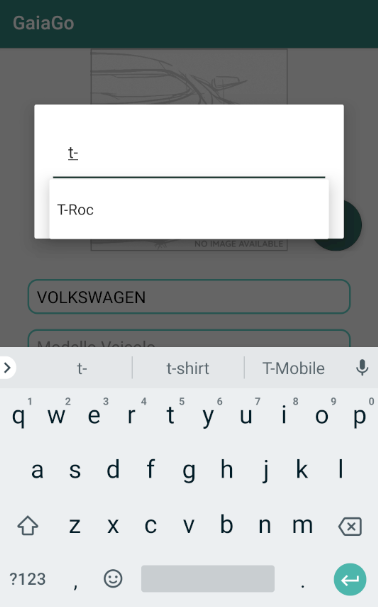
\includegraphics[width=0.5\textwidth]{res/images/modello_auto.png}\\
	\caption{Scelta modello}
	\label{modello}
\end{figure}

\item \textbf{Anno Immatricolazione}: in questa sezione si sceglie l'anno di immatricolazione del proprio veicolo tramite un semplice editor di testo che non viene riportato in figura;
\pagebreak

\item \textbf{Indirizzo}: in questa sezione si inserisce l'indirizzo dove si trova il proprio veicolo, l'indirizzo è geo-localizzato grazie all'uso di un tool\glosp offerto da \textit{Google} il quale ci permette in seguito di ricercare i veicoli in base alla loro posizione sulla mappa. Anche qui è presente l'auto completamento quindi possono essere inseriti solo indirizzi validi altrimenti non sarà possibile localizzare la reale posizione del veicolo;
 \begin{figure}[H] 
	\centering 
	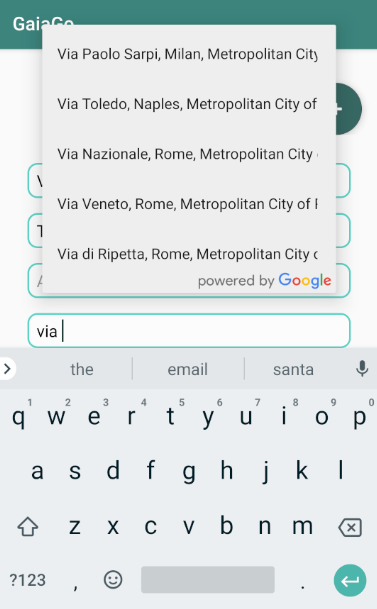
\includegraphics[width=0.5\textwidth]{res/images/indirizzo_auto.png}\\
	\caption{Scelta indirizzo}
	\label{indirizzo}
\end{figure}
\end{itemize}
Per completare l'inserimento è necessario aver compilato tutti i campi richiesti quindi si preme il bottone verde "REGISTRA VEICOLO"
\pagebreak

\subsubsection{Ricerca veicolo}
\label{sec:hello}

Per effettuare una prenotazione è necessario ricercare i veicoli resi disponibili dagli altri utenti. Per fare ciò da una delle schermate principali si clicca il pulsante sulla barra di navigazione avente una lente d'ingrandimento stilizzata. Una volta premuto veniamo trasferiti nell'attività principale di ricerca, il bottone nella barra di navigazione presenta ora una scritta "Cerca" a conferma di ciò.
  \begin{figure}[H] 
 	\centering 
 	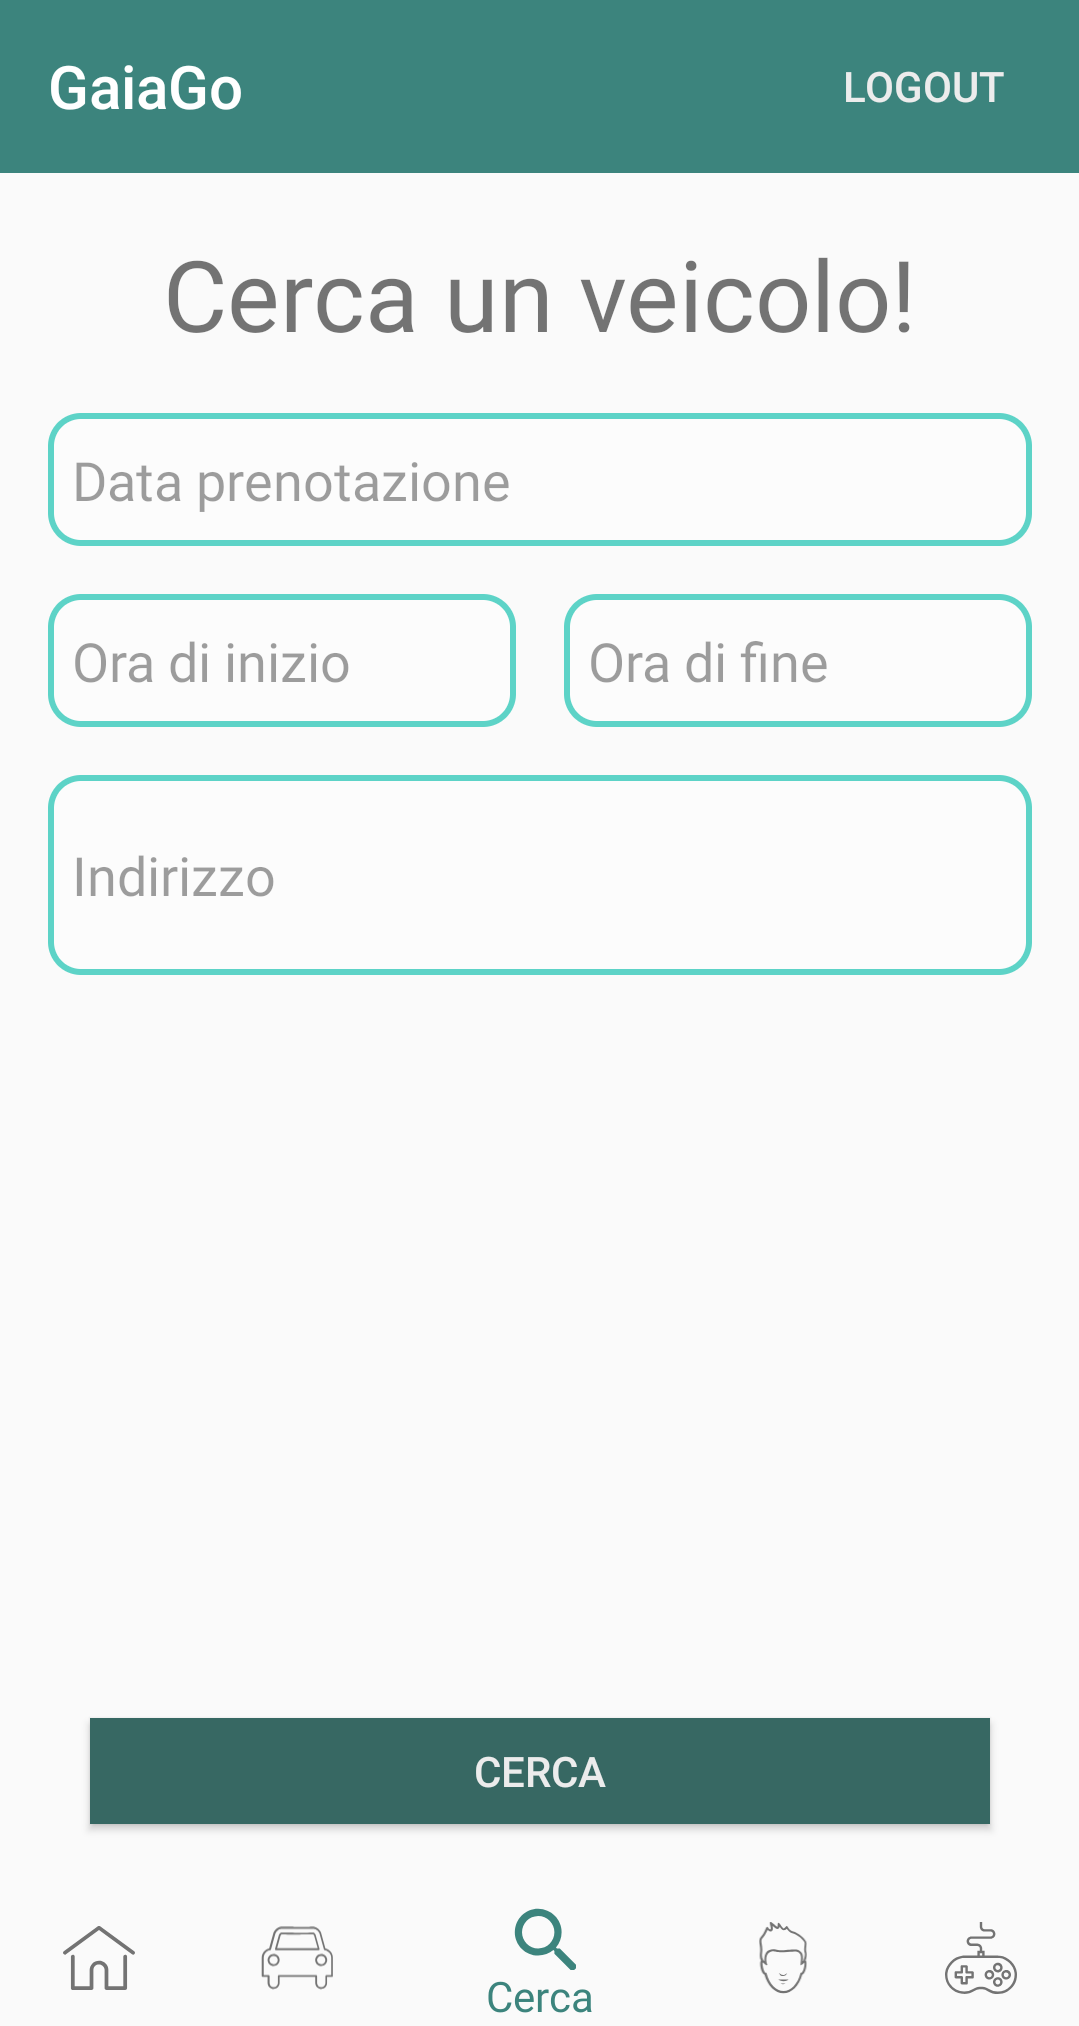
\includegraphics[width=0.5\textwidth]{res/images/cerca_veicolo.png}\\
 	\caption{Activity di ricerca veicolo}
 	\label{ricerca}
 \end{figure}
\pagebreak

Per effettuare una ricerca è necessario compilare tutti i campi richiesti:
\begin{itemize}
	\item \textbf{Data Prenotazione}: è richiesto il giorno in cui si intende effettuare la prenotazione, per fare ciò si clicca sull'editor di testo avente il placeholder\glosp "Data prenotazione" in grigio chiaro. Compare un calendario nel quale si va a selezionare il giorno voluto;
	 \begin{figure}[H] 
	 	\centering 
	 	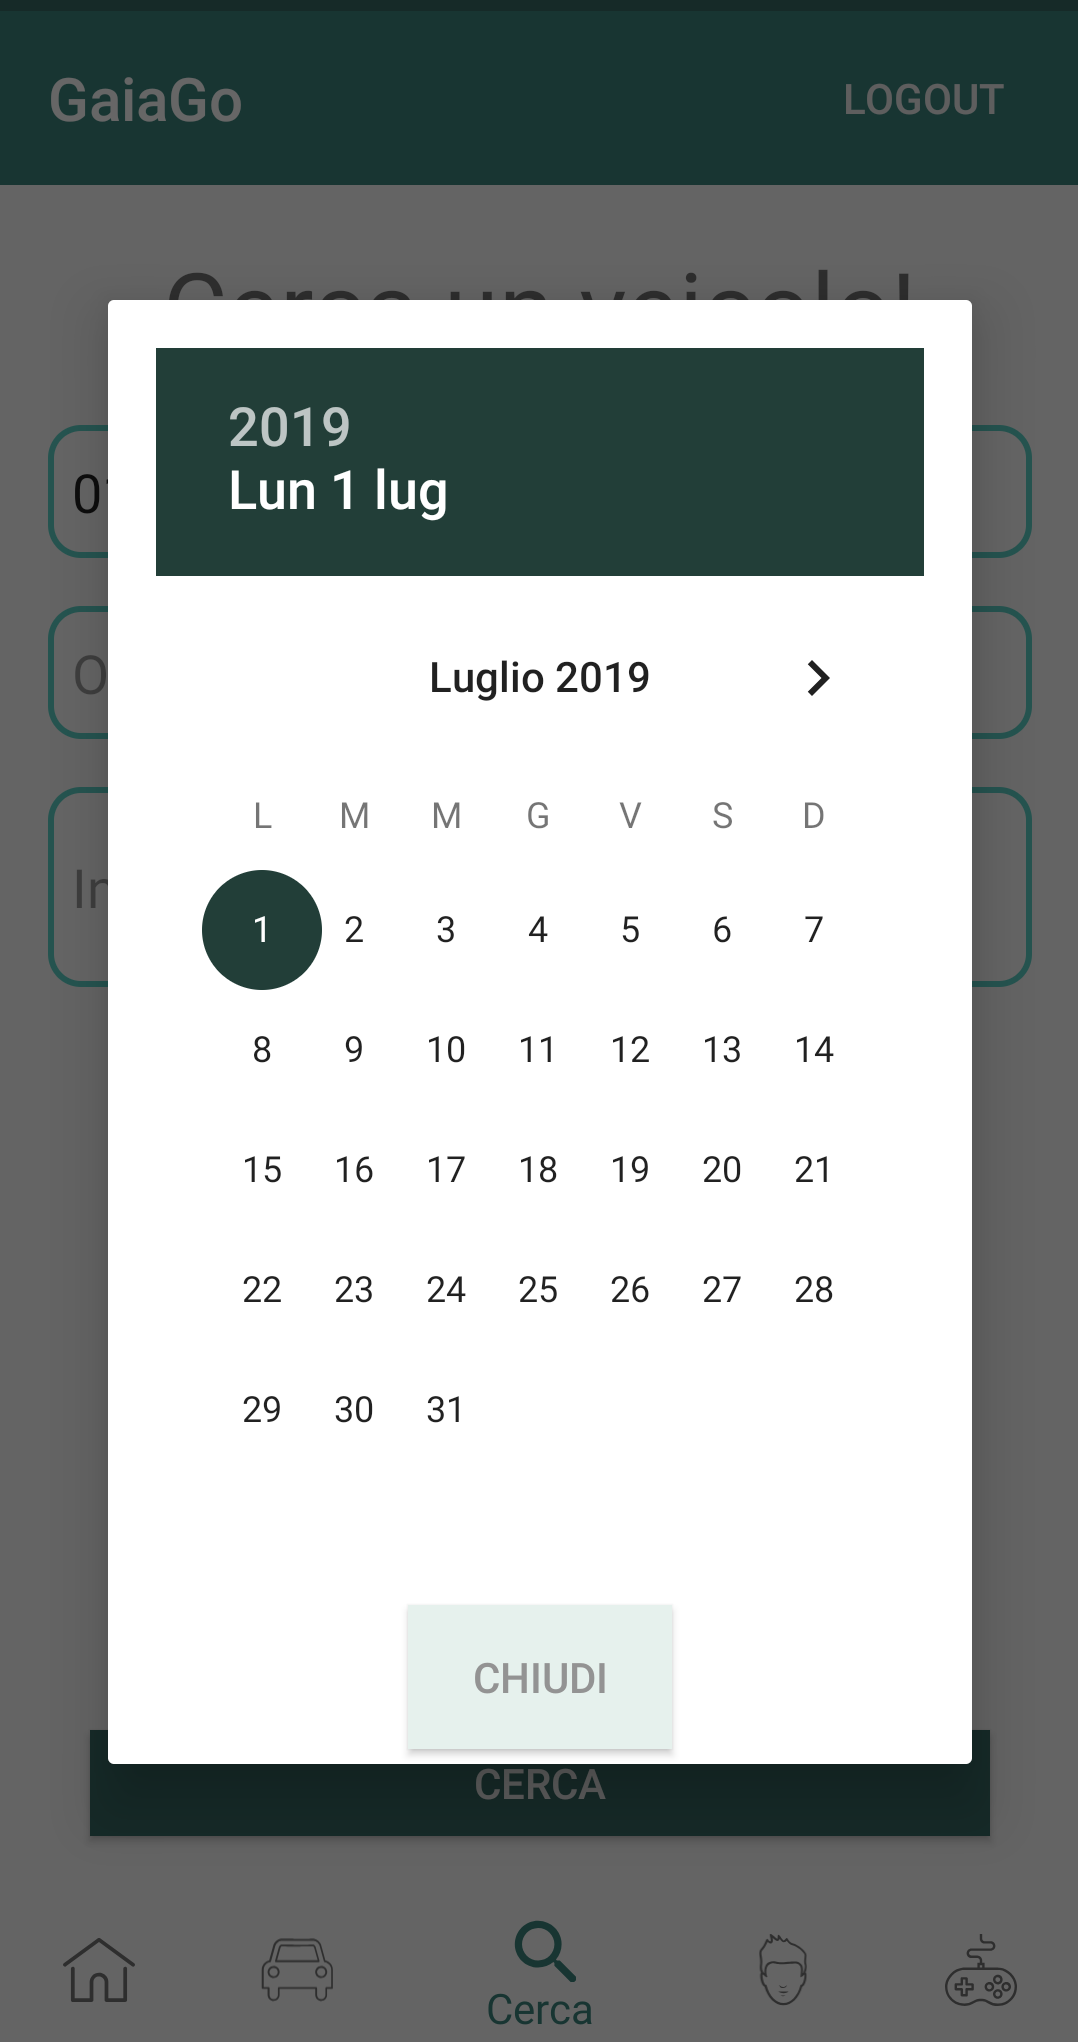
\includegraphics[width=0.5\textwidth]{res/images/data_prenotazione.png}\\
	 	\caption{Data prenotazione}
	 	\label{data}
	 \end{figure}
 \pagebreak
 
 \item \textbf{Ora di Inizio/Fine}: è necessario inserire la fascia oraria nella quale si intende prenotare il veicolo, per fare ciò sono disponibili due campi compilabili "Ora inizio" e "Ora fine". Una volta cliccati presentano gli orari da scegliere con una sensibilità di 15 minuti;
  \begin{figure}[H] 
 	\centering 
 	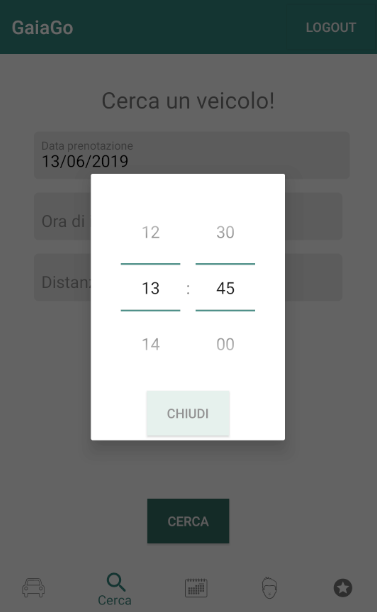
\includegraphics[width=0.5\textwidth]{res/images/ora_inizio.png}\\
 	\caption{Ora prenotazione}
 	\label{ora}
 \end{figure}
 
 \item \textbf{Distanza in Km}: è necessario inserire la distanza del raggio in cui si vuole ricercare un veicolo, per fare ciò si completa un semplice campo "Distanza in km" con un numero intero.
\end{itemize}
\pagebreak

Dopo aver compilato tutti i campi si preme il bottone "CERCA" di colore verde e si viene portati alla seguente schermata:
  \begin{figure}[H] 
	\centering 
	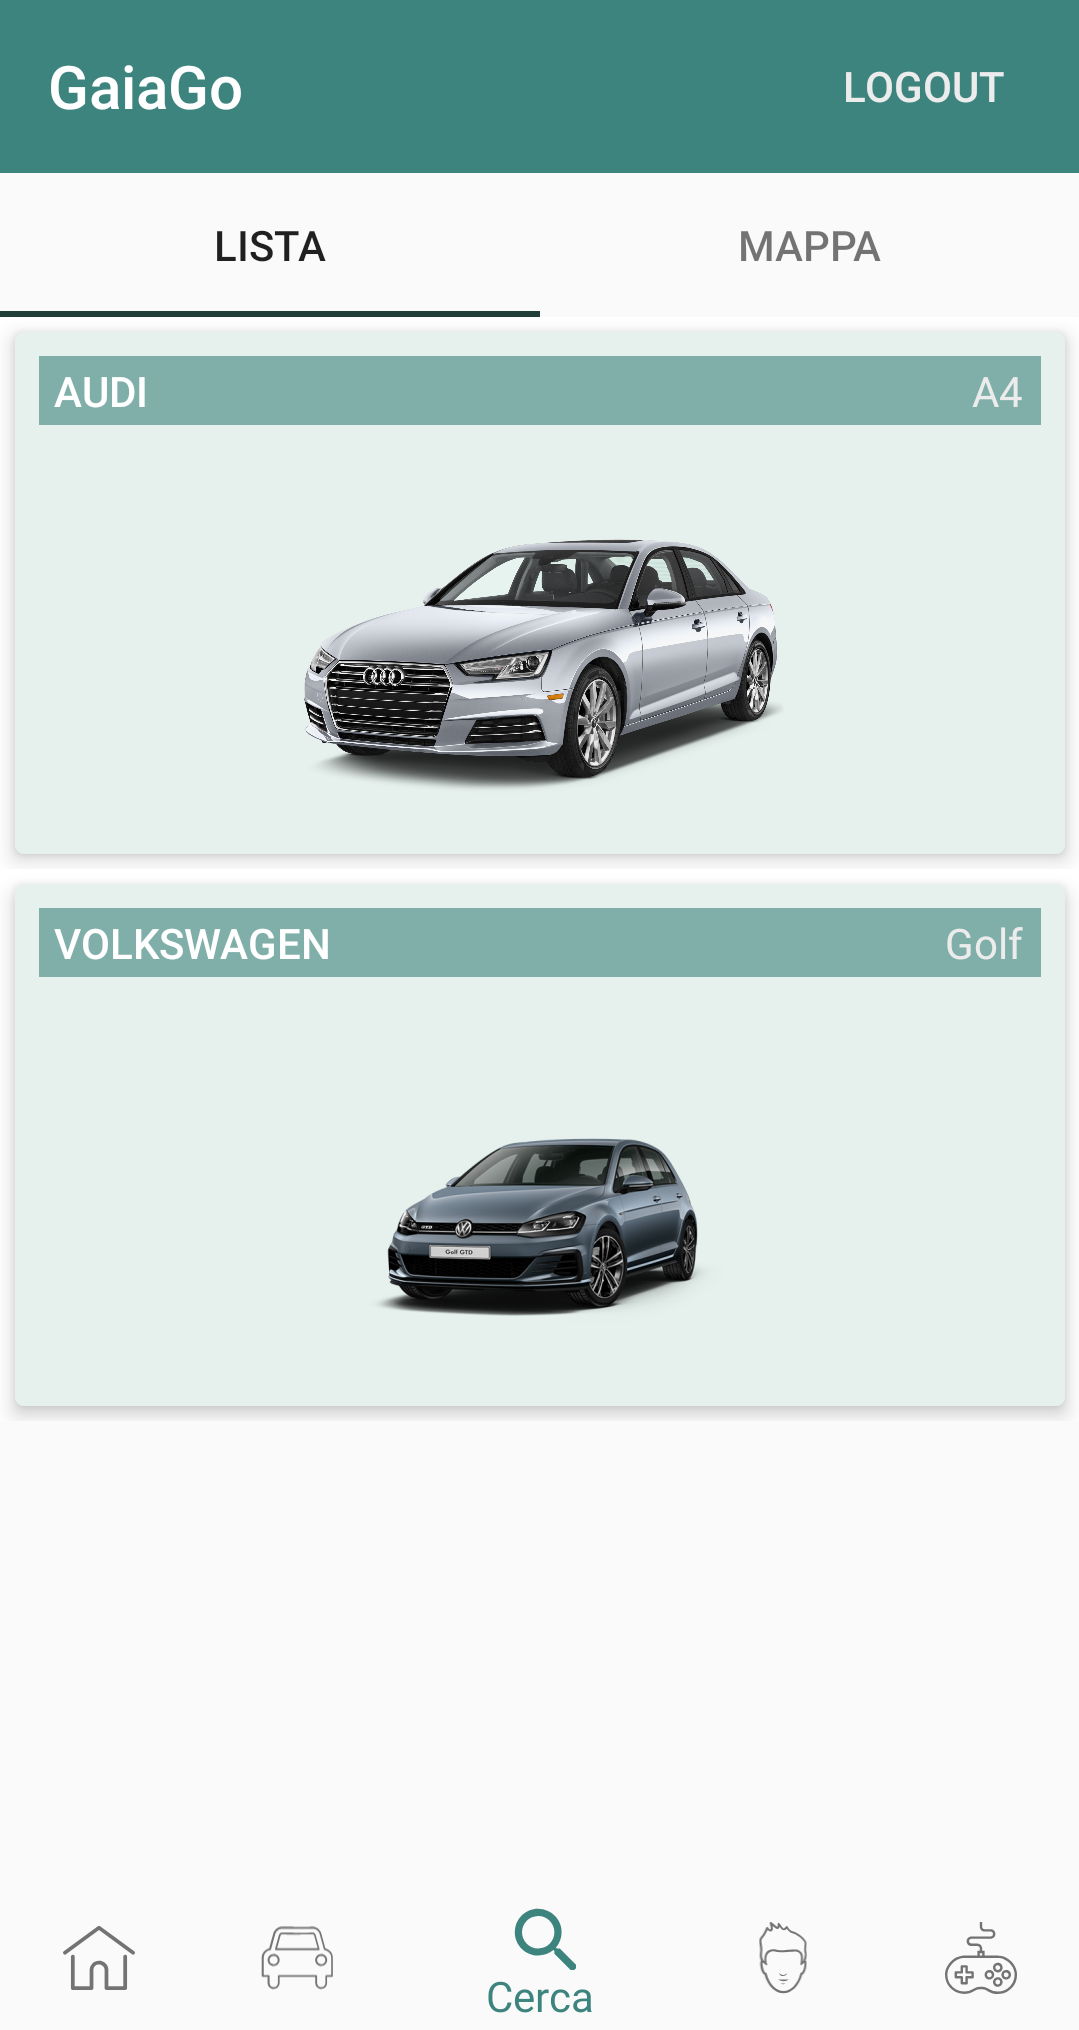
\includegraphics[width=0.5\textwidth]{res/images/ricerca_conclusa.png}\\
	\caption{Ricerca conclusa}
	\label{conclusa}
\end{figure}
\pagebreak

Per scegliere quale auto prenotare si clicca in qualsiasi punto all'interno del riquadro dell'auto desiderata e si viene portati alla seguente schermata:
  \begin{figure}[H] 
	\centering 
	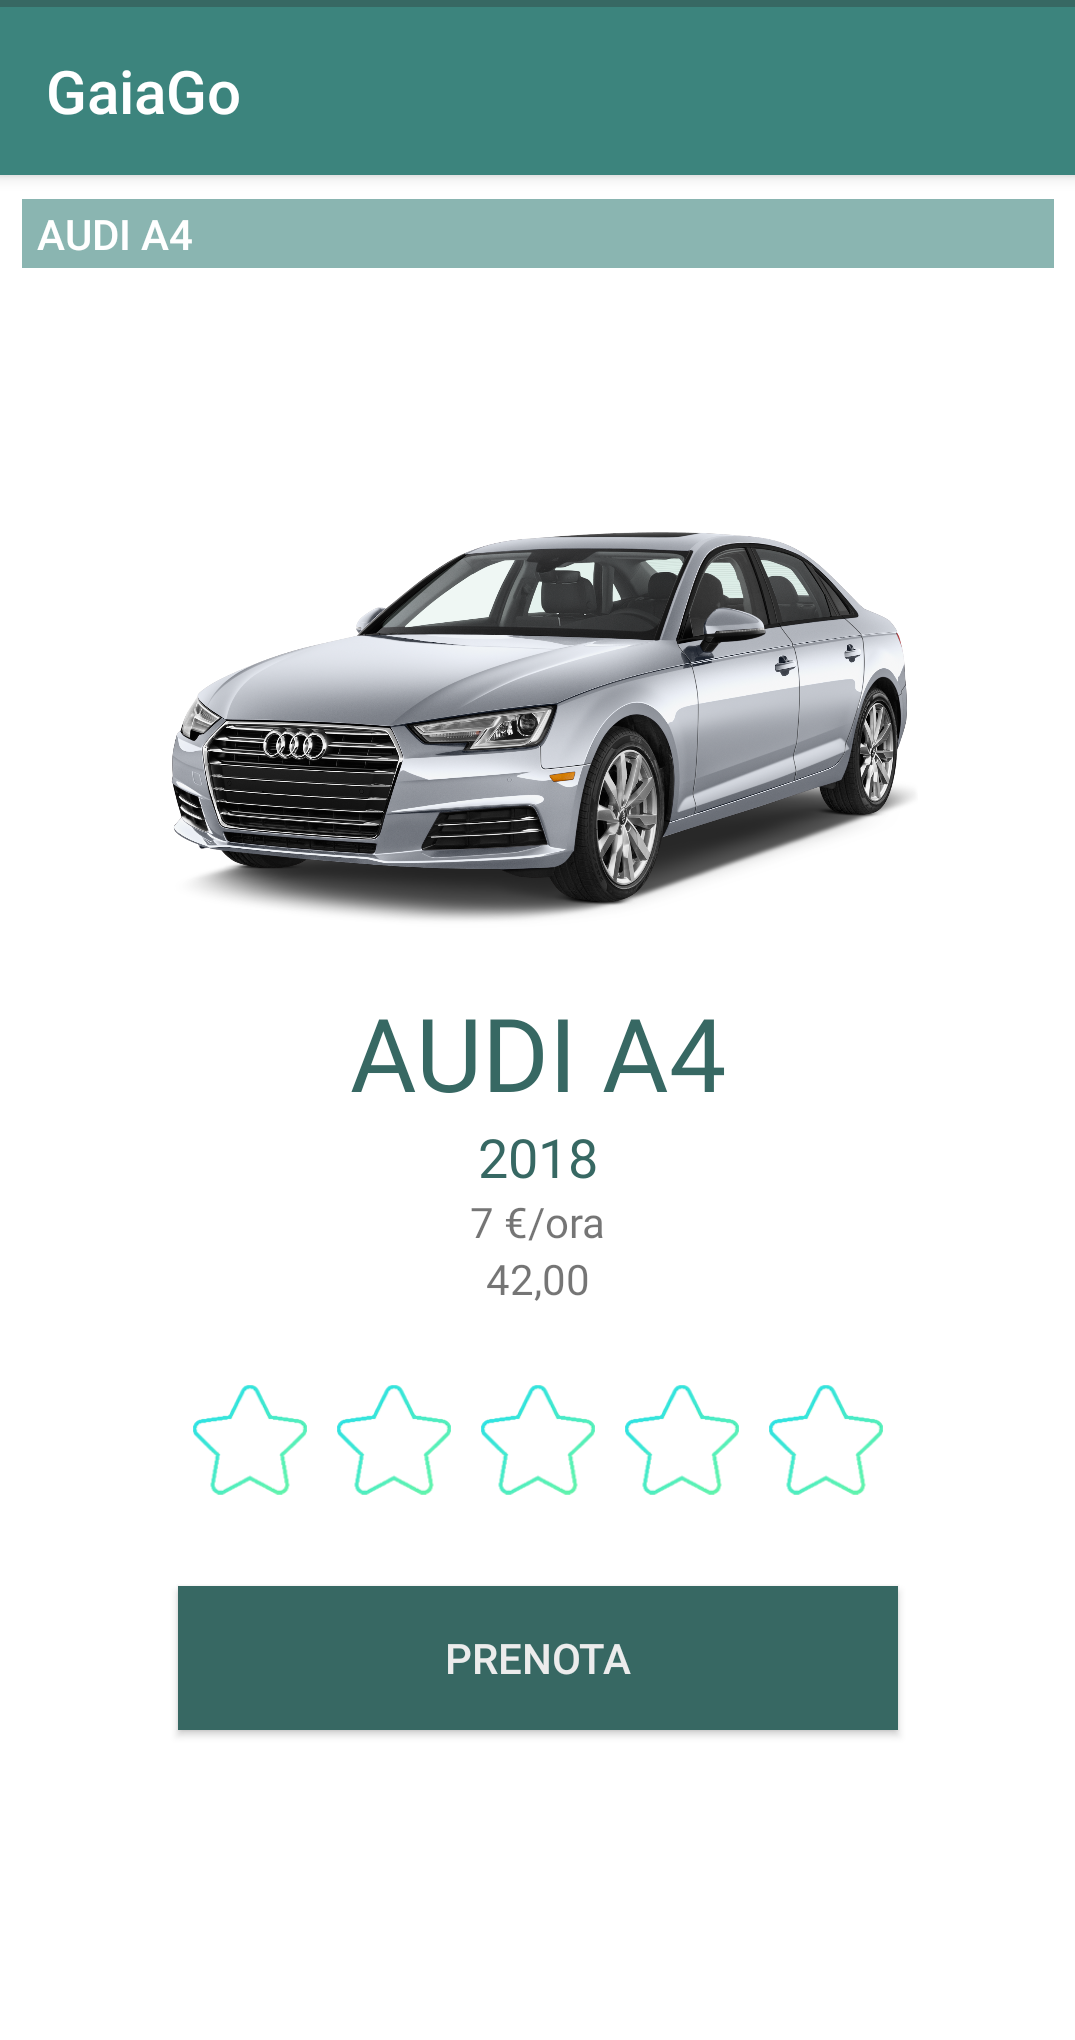
\includegraphics[width=0.5\textwidth]{res/images/prenotazione1.png}\\
	\caption{Auto scelta}
	\label{scelta}
\end{figure}
Qui sono riportati la foto, anno di immatricolazione e il rating\glosp ricevuto dagli utenti che ne hanno fatto utilizzo. Per richiedere la prenotazione si preme sul pulsante verde "PRENOTA".
\pagebreak

\subsection{Gestione prenotazioni}
Nell'attività di gestione delle prenotazioni l'utente può vedere i veicoli che ha prenotato e/o i suoi veicoli che sono stati prenotati da altri, per accedervi basta premere nella barra di navigazione il pulsante con un calendario stilizzato, una volta premuto compare la scritta "Prenotazioni".
  \begin{figure}[H] 
	\centering 
	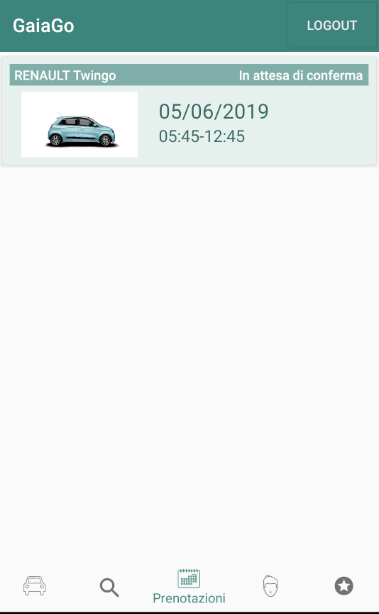
\includegraphics[width=0.5\textwidth]{res/images/prenotazione3.png}\\
	\caption{Lista auto prenotate}
	\label{prenotate}
\end{figure}
\pagebreak

Ora suddividiamo le prenotazioni in base al tipo:
\begin{itemize}
	\item \textbf{Utente}: dopo aver prenotato un veicolo tramite la ricerca questo sarà presente nella schermata sopracitata, se si va a cliccare sul riquadro corrispondente si apre una nuova sotto-attività nella quale è possibile vedere il dettaglio della prenotazione, comprendente gli orari, giorno e stato il quale viene modificato se il proprietario accetta. È inoltre possibile annullare la prenotazione tramite il tasto "ANNULLA PRENOTAZIONE";
	  \begin{figure}[H] 
		\centering 
		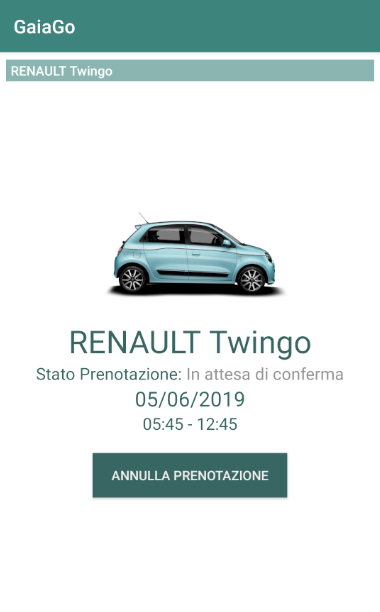
\includegraphics[width=0.5\textwidth]{res/images/prenotazione2.png}\\
		\caption{Auto prenotata}
		\label{prenotata}
	\end{figure}
\pagebreak
	\item \textbf{Proprietario}: dopo aver messo a disposizione un veicolo perché venga prenotato, ed un utente ne richiede la prenotazione, nella schermata contenente tutte le prenotazioni è possibile cliccare sulla propria auto e si viene condotti alla schermata per la conferma o rifiuto della prenotazione, contiene inoltre tutti i dati riguardanti gli orari e il giorno richiesti.
	  \begin{figure}[H] 
		\centering 
		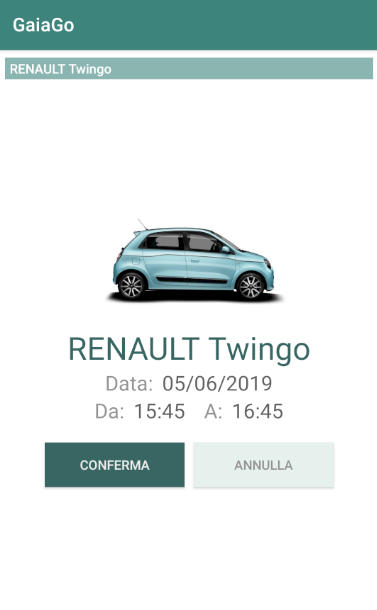
\includegraphics[width=0.5\textwidth]{res/images/conferma_prenotazione.png}\\
		\caption{Richiesta di prenotazione}
		\label{prenotazione}
	\end{figure}
\end{itemize}
\pagebreak

\subsection{Inserimento Disponibilità}
Nella schermata principale di visualizzazione dei veicoli è possibile, cliccando su uno di essi, vedere i dettagli di quest'ultimo e si ha la possibilità di rimuoverlo dall'applicazione oppure di aggiungerlo alle prenotazioni. Una volta presenti nella schermata del veicolo si clicca sul pulsante "AGGIUNGI DISPONIBILITÀ".
	  \begin{figure}[H] 
	\centering 
	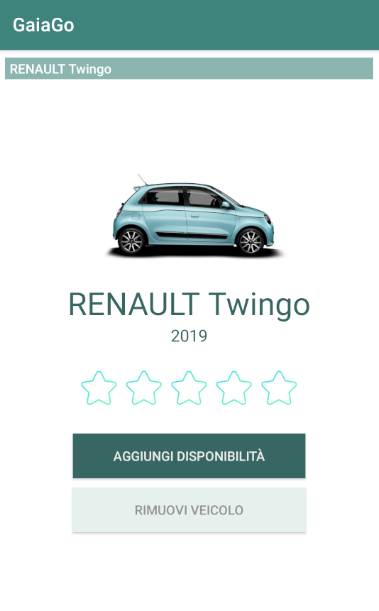
\includegraphics[width=0.5\textwidth]{res/images/aggiungi_disponibilita1.png}\\
	\caption{Aggiunta disponibilità}
	\label{disponibilità}
\end{figure}
\pagebreak

Una volta premuto il pulsante si passa all'attività di inserimento dei dati per definire i giorni e la fascia oraria in cui sarà possibile richiedere una prenotazione del veicolo. Premendo sul campo "Data prenotazione" si avrà accesso ad un calendario per indicare il giorno un cui rendere disponibile il mezzo, "Ora inizio" e "Ora fine" richiedono l'inserimento di una fascia oraria con uno scarto di 15 minuti.
Le azioni sopracitate sono analoghe alla ricerca di una prenotazione, si rimanda alla sezione \textit{\hyperref[sec:hello]{Ricerca veicolo}} per la spiegazione con annesse figure.
 \begin{figure}[H] 
	\centering 
	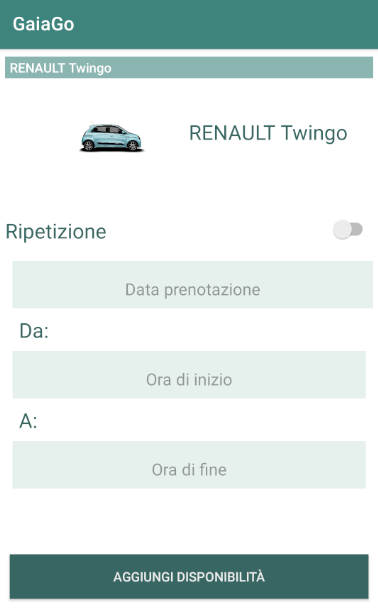
\includegraphics[width=0.5\textwidth]{res/images/aggiungi_disponibilita2.png}\\
	\caption{Inserimento campi disponibilità}
	\label{campi disponibilità}
\end{figure}
\pagebreak

Si presti particolare attenzione al tasto posto a destra di "Ripetizione", il quale da accesso ad un nuovo insieme di campi per poter rendere disponibile il veicolo più volte senza dover inserire manualmente tutti i dati. Si presuma che l'utente proprietario voglia rendere prenotabile il proprio mezzo tutti i martedì dalle 10:00 alle 13:00 con questa schermata può farlo una sola volta anziché doverlo inserire per ogni settimana.

 \begin{figure}[H] 
	\centering 
	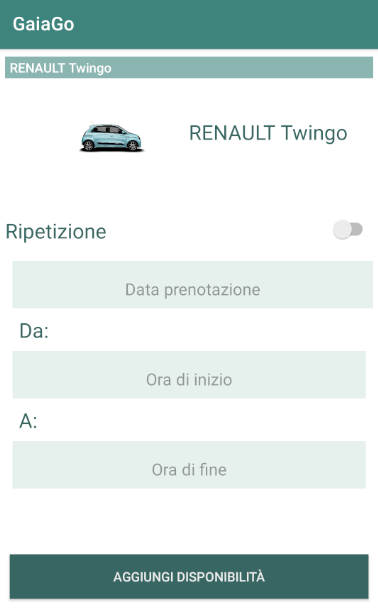
\includegraphics[width=0.5\textwidth]{res/images/aggiungi_disponibilita2.png}\\
	\caption{Ripetizione disponibilità}
	\label{disponibilità2}
\end{figure}
Una volta compilati tutti i campi è necessario premere il bottone "AGGIUNGI DISPONIBILITÀ" per completare l'azione.
\pagebreak

\subsection{Profilo Utente}
Questa sezione include tutti i dati dell'utente corrente. Presenta la patente, nome e cognome, numero di cellulare, email, data di nascita e indirizzo di residenza.
 \begin{figure}[H] 
	\centering 
	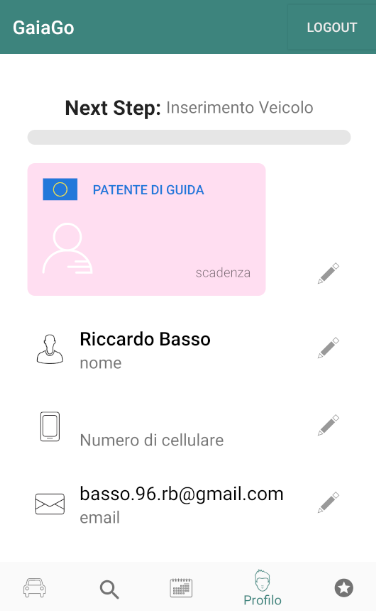
\includegraphics[width=0.5\textwidth]{res/images/profilo_utente.png}\\
	\caption{Profilo utente}
	\label{profilo}
\end{figure}
\pagebreak

Ogni campo risulta modificabile, di seguito è mostrato passo passo la procedura da seguire per ognuno:
\begin{itemize}
	\item \textbf{Patente di guida}: cliccando sull'icona a forma di penna a destra dell'immagine della patente si passa alla fase di inserimento e modifica;
	 \begin{figure}[H] 
		\centering 
		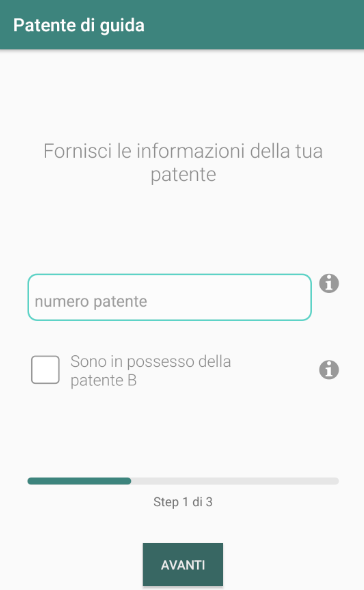
\includegraphics[width=0.5\textwidth]{res/images/patente1.png}\\
		\caption{Patente}
		\label{patente}
	\end{figure}
\pagebreak

È necessario compilare il campo numero patente, l'utente può ricevere un aiuto premendo il tasto info posto a destra.
 \begin{figure}[H] 
 	\centering 
 	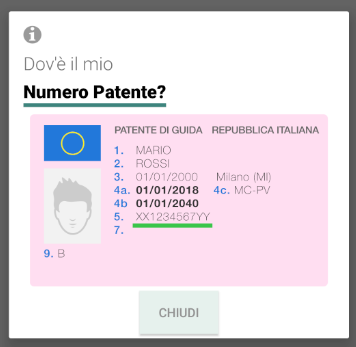
\includegraphics[width=0.5\textwidth]{res/images/patente1_info.png}\\
 	\caption{Info numero patente}
 	\label{patente1}
 \end{figure}
L'errore che si prensenta nel caso in cui non venga inserito il numero è il seguente:
 \begin{figure}[H] 
	\centering 
	
\includegraphics[width=0.5\textwidth]{res/images/patente1errore.png}\\
	\caption{Errore numero patente}
	\label{patenteerror}
\end{figure}
\pagebreak

Per inserire la patente è necessario essere in possesso della patente di grado B, un altra info è disponibile cliccando la relativa icona posta a destra.
\begin{figure}[H] 
	\centering 
	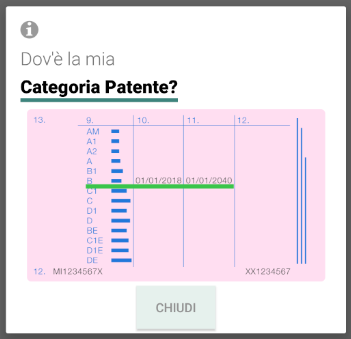
\includegraphics[width=0.5\textwidth]{res/images/patente1_info2.png}\\
	\caption{Info patente B}
	\label{patente2}
\end{figure}
\pagebreak

Al termine dell'inserimento dei dati la schermata si presenta nel modo seguente:
\begin{figure}[H] 
	\centering 
	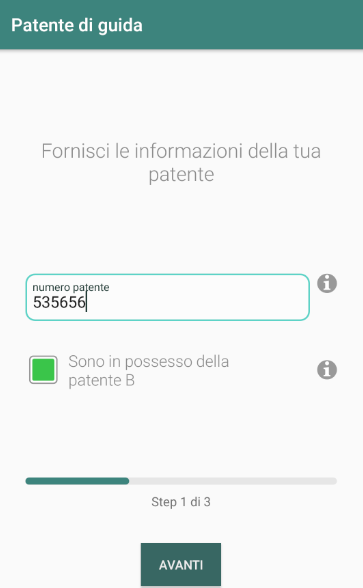
\includegraphics[width=0.5\textwidth]{res/images/patente1_1.png}\\
	\caption{Schermata completata con i relativi campi}
	\label{patente3}
\end{figure}
Per proseguire si prema il pulsante "AVANTI".
\pagebreak

Il prossimo step di inserimento richiede la data di rilascio e la data di scadenza compilabili tramite un calendario come già visto in precedenza.
\begin{figure}[H] 
	\centering 
	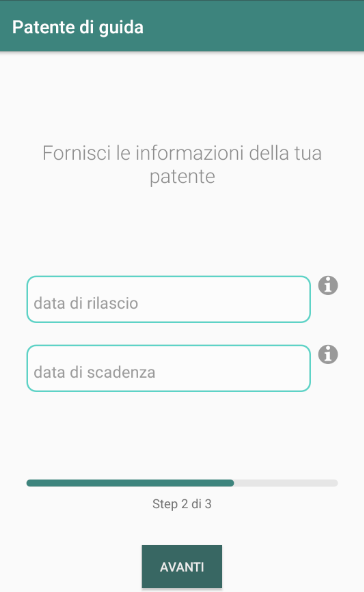
\includegraphics[width=0.5\textwidth]{res/images/patente2.png}\\
	\caption{Seconda schermata patente}
	\label{patente4}
\end{figure}
\pagebreak

Anche in questa sezione sono presenti degli aiuti all'utente per indicare dove cercare le date richieste premendo sul tasto info.
\begin{figure}[H] 
	\centering 
	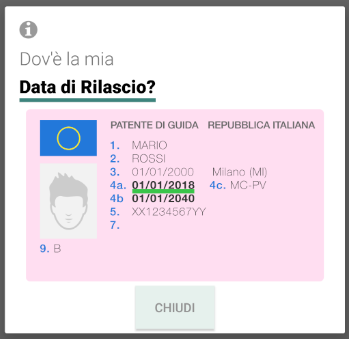
\includegraphics[width=0.5\textwidth]{res/images/patente2_1.png}\\
	\caption{Data di rilascio}
	\label{patente5}
\end{figure}
Errore annesso:
 \begin{figure}[H] 
	\centering 
	
\includegraphics[width=0.5\textwidth]{res/images/patente2errore_rilascio.png}\\
	\caption{Errore data rilascio}
	\label{patenteerror1}
\end{figure}
\begin{figure}[H] 
	\centering 
	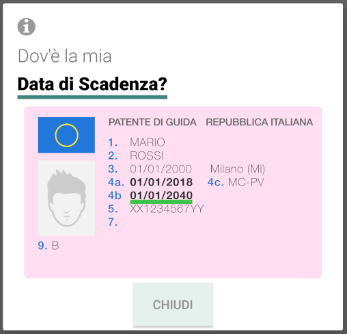
\includegraphics[width=0.5\textwidth]{res/images/patente2_2.png}\\
	\caption{Data di scadenza}
	\label{patente6}
\end{figure}
Errore annesso:
\begin{figure}[H] 
	\centering
	
\includegraphics[width=0.5\textwidth]{res/images/patente2errore_scadenza.png}\\
	\caption{Errore data scadenza}
	\label{patenteerror2}
\end{figure}
\pagebreak

Il prossimo step di inserimento richiede la foto fronte e retro della patente.
\begin{figure}[H]
	\centering
	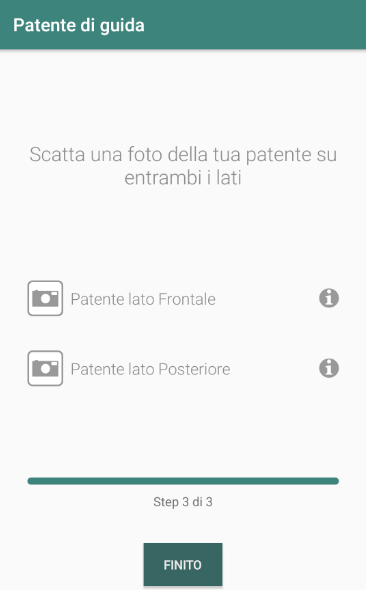
\includegraphics[width=0.5\textwidth]{res/images/patente3.png}\\
	\caption{Foto patente}
	\label{patente7}
\end{figure}
\pagebreak

Anche in questa sezione sono presenti degli aiuti all'utente per indicare quale lato inserire premendo sul tasto info.
\begin{figure}[H] 
	\centering 
	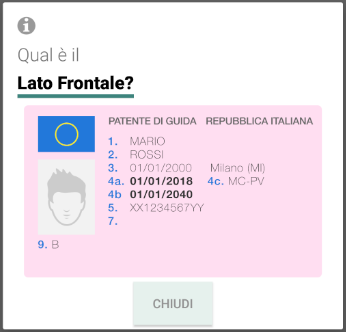
\includegraphics[width=0.5\textwidth]{res/images/patente3_1.png}\\
	\caption{Lato frontale}
	\label{patente8}
\end{figure}
Errore annesso:
\begin{figure}[H] 
	\centering 
	
\includegraphics[width=0.5\textwidth]{res/images/patente3errore_front.png}\\
	\caption{Errore foto frontale}
	\label{patenteerror3}
\end{figure}
\pagebreak

\begin{figure}[H] 
	\centering 
	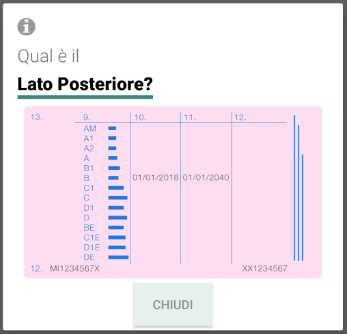
\includegraphics[width=0.5\textwidth]{res/images/patente3_2.png}\\
	\caption{Lato posteriore}
	\label{patente9}
\end{figure}
Errore annesso:
\begin{figure}[H] 
	\centering 
	
\includegraphics[width=0.5\textwidth]{res/images/patente3errore.png}\\
	\caption{Errore foto posteriore}
	\label{patenteerror4}
\end{figure}
\pagebreak

	\item \textbf{Nome e cognome}: cliccando sull'icona a forma di penna a destra del nome si passa alla fase di inserimento e modifica;
	\begin{figure}[H] 
		\centering 
		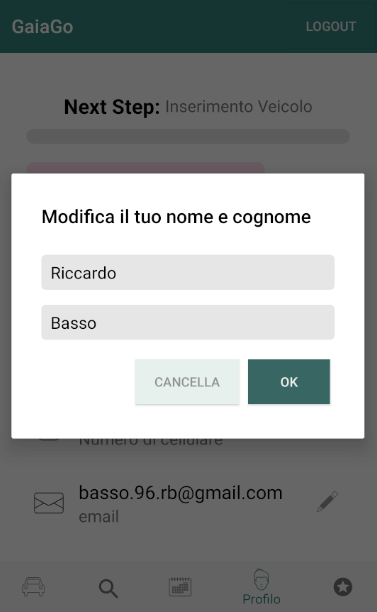
\includegraphics[width=0.5\textwidth]{res/images/modifica_nome.png}\\
		\caption{Modifica del nome}
		\label{modificanome}
	\end{figure}
\pagebreak

		\item \textbf{Numero di cellulare}: cliccando sull'icona a forma di penna a destra del numero di cellulare si passa alla fase di inserimento e modifica;
	\begin{figure}[H] 
		\centering 
		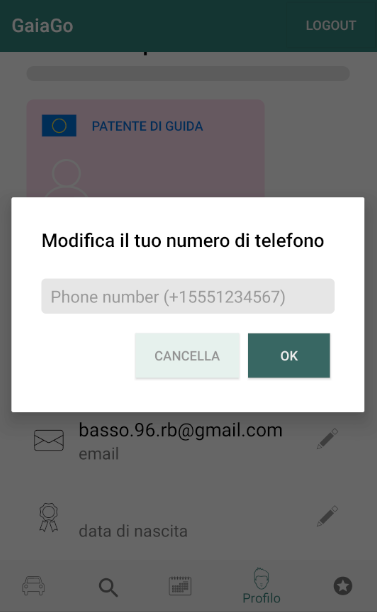
\includegraphics[width=0.5\textwidth]{res/images/modifica_cellulare.png}\\
		\caption{Modifica del cellulare}
		\label{modificell}
	\end{figure}
\pagebreak

\item \textbf{Data di nascita}: cliccando sull'icona a forma di penna a destra della data di nascita si passa alla fase di inserimento e modifica;
\begin{figure}[H] 
	\centering 
	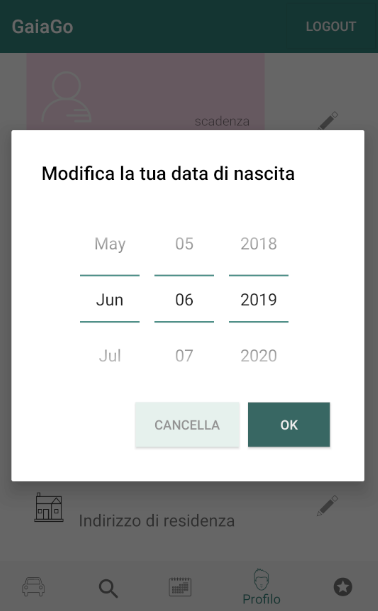
\includegraphics[width=0.5\textwidth]{res/images/modifica_data_nascita.png}\\
	\caption{Data di nascita}
	\label{modificanascita}
\end{figure}
\pagebreak

\item \textbf{Residenza}: cliccando sull'icona a forma di penna a destra della residenza si passa alla fase di inserimento e modifica;
\begin{figure}[H] 
	\centering 
	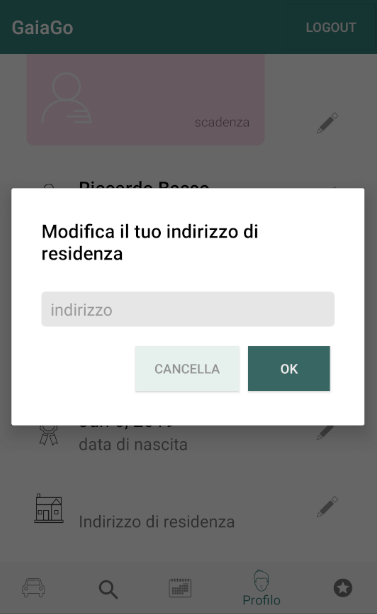
\includegraphics[width=0.5\textwidth]{res/images/modifica_residenza.png}\\
	\caption{Modifica della residenza}
	\label{modifiresidenza}
\end{figure}
\pagebreak
\end{itemize}
	
